\begin{frame}
\frametitle{Définitions Fondamentales des Graphes}

\begin{tcolorbox}[colback=orange!10,colframe=orange!100!black,
    title=Un Graphe]
    Un \textbf{graphe} est un ensemble de sommets et d'arêtes
\end{tcolorbox}

\begin{tcolorbox}[colback=orange!10,colframe=orange!100!black,
    title=Les Sommets]
    Les \textbf{sommets} (ou nœuds) représentent les entités du graphe.
\end{tcolorbox}


\begin{tcolorbox}[colback=orange!10,colframe=orange!100!black,
    title=Les Arêtes]
    Les \textbf{arêtes} (ou liens) représentent les relations entre les sommets.
\end{tcolorbox}

\begin{figure}[H]
    \centering
    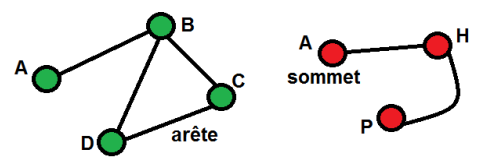
\includegraphics[width=0.35 \textwidth]{Figures/graphes.PNG}
    \caption{Graphe non Orienté}
    \label{fig:Graphe , Sommets , Aretes}
\end{figure}

\end{frame}
